\documentclass[]{subfiles}

\begin{document}


\begin{landscape}
    \section{Design}
	\subsection{Domänenmodell}
	\begin{figure}[h!]
		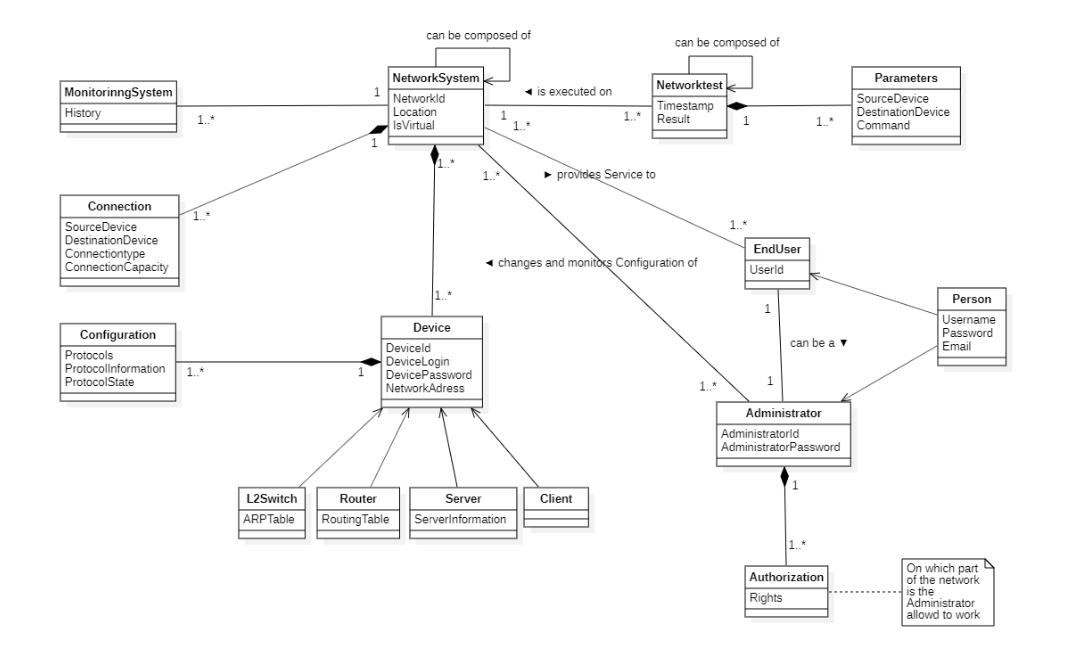
\includegraphics[scale = 0.6]{\vorlagenOrdner/Bilder/DomainModell}
		\caption{Domainmodell}
	\end{figure}
	\newpage	
\end{landscape}


	\subsubsection{Prosa}
	Ein Netzwerk (Network System) setzt sich aus mindestens zwei Geräten (Device) und Verbindungen dazwischen (Connection) zusammen.
	Es kann auch mehrere Teilnetzwerke in sich vereinen, z.B die beiden Netzwerke aus Haupt- und Nebengebäude ergeben das gesamte Firmennetzwerk.
	Das Netzwerksystem kann auch in virtueller Form aufgebaut sein, Beispielsweise als Netz von virtuellen Routern auf einem Server.
	Ein Device kann in die vier Kategorien Switch, Router (Level-3-Switch), Server und Client eingeteilt werden und hat eine oder mehrere Konfigurationen.
	Beispielsweise kann ein Router das OSPF (Open Shortest Path First) Protokoll und zusätzlich als Fallback statische Routen konfiguriert haben.

	Geräte haben eine Identifikation, ein Gerätelogin und -passwort und eine Addresse innerhalb des Netzwerkes.
	Die Konfiguration der Geräte setzt sich zusammen aus dem Protokoll, dessen Informationen und dem Zustand, in dem das Gerät mit dem Protokoll gerade ist.

	Es ist möglich, dass ein Netzwerksystem ein Monitoring System hat, das die Zustände zur Laufzeit überwacht, z.B. Welche Verbindungen gerade aktiv sind und wieviele Client auf dem Netzwerksystem angemeldet sind.
	Das Monitoring speichert auch vergangene Daten in einer Historie, so dass vergangene Zustände mit dem aktuellen Zustand verglichen werden können.

	Netzwerktests, wie sie von Netzwerk-Technikern auf dem Netzwerk ausgeführt werden, haben Parameter und können aus weiteren Tests zusammengesetzt sein. 
	Ein umfangreicher Systemtest kann aus mehreren Ping-Tests bestehen.
	Ein Netzwerktest umfasst einen Zeitstempel, um die genaue Durchführungszeit ermitteln zu können und hat ein Resultat, üblicherweise bestanden oder durchgefallen.
	Die Parameter eines Netzwerktests sind üblicherweise ein Befehl (Ping, Traceroute etc.) und ein Source- und/oder Destination-Device.

	Auf dem Netzwerksystem arbeiten verschiedene Personen. 
	Jede Person benötigt einen Usernamen, ein Passwort und eine E-Mail-Addresse, um sich gegenüber dem Neztwerk zu authentifizieren.
	Diese können in User und Administratoren eingeteilt werden. 
	Usern werden Services vom Netzwerk wie Internet oder Serverzugriff angeboten, und sie haben eine UserID, mit der sie das Netzwerk erkennt.
	Administratoren können die Konfiguration des Netzwerks einsehen und verändern. 
	Zusätzlich zum regulären Login haben sie einen Administratorzugriff, der aus einer ID und einem Admin-Passwort besteht.
	Dazu benötigen sie eine Authorisierung, um auf dem Netzwerksystem zu arbeiten.

\begin{landscape}
	\subsection{Klassendiagramm}
	\begin{figure}[h!]
			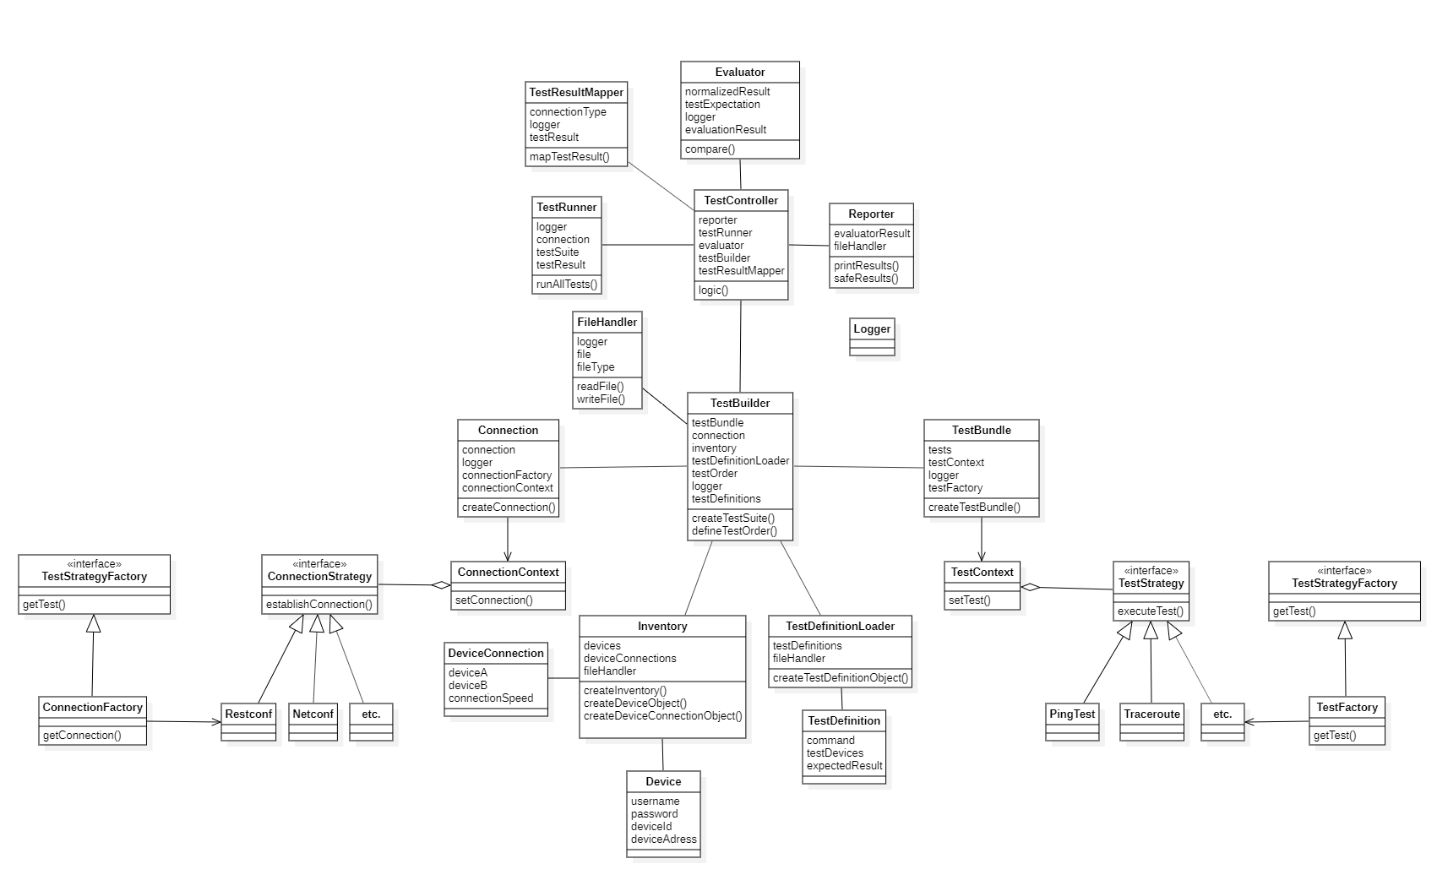
\includegraphics[scale = 0.6]{\vorlagenOrdner/Bilder/Klassendiagramm}
			\caption{Klassendiagramm}
	\end{figure}
	\newpage	
\end{landscape}


	\subsubsection{Beschreibungen}

	\minisec{NetworkTestController}
	Der TestController ist das Kernstück des Programms. 
	Er beinhaltet die Main-Methode und steuert den Ablauf des Programms. 
	Vom TestController werden der TestRunner, der TestBuilder, der Evaluator 
	und der Reporter instanziert und er ist zuständig für die Kommunikation 
	zwischen diesen Komponenten.
	
	\begin{tabularx}{\textwidth}{lX}
		\toprule
			Komponenten & Beschreibung \\
		\midrule
			reporter & Referenz auf die Reporter-Instanz \\
			testRunner & Referenz auf die TestRunner-Instanz \\
			evaluator & Referenz auf die Evaluator-Instanz \\
			testBuilder & Referenz auf die TestBuilder-Instanz \\
		\midrule
			logic() & Methode, die für die Programmausführung sämtliche referenzierten Komponenten instanziert und deren Funktionalität in der korrekten Reihenfolge ausführt.\\
			run() & Main-Methode, die den Testcontroller instanziert. \\
		\bottomrule
	\end{tabularx}

	\minisec{NetworkTestRunner}
	Der TestRunner führt die ihm vom Controller mitgeteilten Tests gemäss der, in der TestSuite angegebenen, Parameter aus. 
	Die zu verwendende Netzwerkschnittstelle (Restconf, Netconf, SSH etc.) wird ihm ebenfalls vom Controller mitgeteilt.
	Die Resultate der Netzwerktests gibt er dem TestController in Form von Rückgabewerten zurück.

	\begin{tabularx}{\textwidth}{lX}
		\toprule
			Komponenten & Beschreibung \\
		\midrule
			logger & Referenz auf die Logger-Instanz \\ 
		\midrule
			runAllTests() & Methode, die die in der Testsuite spezifizierten Tests auf der in der Connection spezifizierten Netzwerkschnittstelle ausführt. \\
		\bottomrule
	\end{tabularx}
	\newpage

	\minisec{TestResultMapper}
	Da die Ergebnisse der Netzwerktests, je nach Betriebssystem des Neztwerkgeräts und Typ der Verbindung (Netconf, Restconf, NAPALM), ein anderes Rückgabeformat hat, müssen die Testresultate normalisiert werden.
	Der TestResultMapper bringt die verschiedenen Rückgabeformate in ein einheitliches Format, welches dem Evaluator für den Ist-, Soll-Vergleich übgeben wird.

	\begin{tabularx}{\textwidth}{lX}
		\toprule
			Komponenten & Beschreibung \\
		\midrule
			connectionType & Der Typ der Connection, mit welchem auf das Netzwerk verbunden wird. \\
			logger & Referenz auf das Logger-Objekt. \\	
			testResult & Die Resultate, welche der TestRunner zurück gibt. \\
		\midrule
			mapTestResult() & Methode, die die Resultate des TestRunners in eine einheitliche Norm bringt. \\
		\bottomrule
	\end{tabularx}

	\minisec{Reporter}
	Der Reporter schreibt die Testergebnisse der fertig ausgeführten Tests auf die Konsole/Benutzeroberfläche und erstellt ein Testprotokoll, welches er über den FileHandler im Directory abspeichert.

	\begin{tabularx}{\textwidth}{lX}
		\toprule
			Komponenten & Beschreibung \\
		\midrule
			evaluationResult & Die Ergebnisse des Evaluators, wie der Soll- Ist-Vergleich der Tests abgelaufen ist. \\
			fileHandler & Referenz auf das FileHandler-Objekt. \\	
		\midrule
			printResults() & Methode die die Testergebnisse auf der Konsole ausgibt. \\
			safeResults() & Methode, die über den FileHandler die Testergebnisse in einem File im Directory abspeichert. \\
		\bottomrule
	\end{tabularx}

	\minisec{Evaluator}
	Der Evaluator vergleicht die ihm vom Controller mitgeteilten Testresultate mit den Testerwartungswerten und evaluiert, ob die Tests bestanden sind oder nicht.

	\begin{tabularx}{\textwidth}{lX}
		\toprule
			Komponenten & Beschreibung \\
		\midrule
			testRunnerResult & Ergebnisse der auf dem Netzwerk vom Runner ausgeführten Tests. \\
			testExpectation & Zu erwartende Ergebnisse für einen spezifischen Test der Testsuite. \\
			logger & Referenz auf das Logger-Objekt. \\
			evaluationResult & Resultat des Soll-Ist-Vergleichs, welches dem Controller zurückgegeben wird.\\
		\midrule
			compare() & Methode, die testRunnerResult mit testExpectation vergleicht und entscheidet, ob der Test erfolgreich war, oder gescheitert ist. \\
		\bottomrule
	\end{tabularx}
	\newpage

	\minisec{FileHandler}
	Der FileHandler ist eine Utility-Klasse, die für das Einlesen und Schreiben von Daten aus dem Programm in das Directory zuständig ist.
	
	\begin{tabularx}{\textwidth}{lX}
		\toprule
			Komponenten & Beschreibung \\
		\midrule
			logger & Referenz auf das Logger-Objekt. \\
			file & Pfad zu dem zu lesenden/schreibenden File. \\
			fileType & Typ des Files, YAML, XML, JSON usw. \\
		\midrule
			readFile() & Methode, die ein vorgegebenes File öffnet und deren Inhalt in das Programm einliest. \\
			writeFile() & Methode, die einen vorgegebenen Text aus dem Programm in ein File im Directory schreibt. \\
		\bottomrule
	\end{tabularx}

	\minisec{Testbuilder}
	Der Testbuilder ist für die Zusammenstellung der Tests verantwortlich. 
	Er instanziert einen TestDefinitionLoader, der aus dem TestDefinitionsDirectory, worin mehrere Files mit TestDefinitionen gespeichert sind, die einzelnen TestDefinitionen ausliest.
	Dann holt er sich aus dem Inventory die Devices und deren Connections. 
	Die TestDefinitionen attributisiert er mit den, in der TestStrategy definierten Tests, und erstellt mit den Parametern aus dem Inventar das TestBundle. 
	Hier kann vom Benutzer auch die Auswahl der einzelnen Tests, welche durchgeführt werden sollen, sowie die Durchführungsreihenfolge festgelegt werden.
	Die Connection spezifiziert die konkrete Netzwerkschnittstelle, über welche die Netzwerktests vom Runner dann durchgeführt werden sollen.

	\begin{tabularx}{\textwidth}{lX}
		\toprule
			Komponenten & Beschreibung \\
		\midrule
			testBundle & Collection von Tests mit Parametern für die Ausführung als Referent auf ein TestBundle-Objekt. \\
			connection & Referenz auf das Connection-Objekt. \\
			inventory & Referenz auf das Inventory-Objekt. \\
			testDefinitionLoader & Referenz auf ein TestDefinitionLoader-Objekt.\\
			testOrder & Definition, in welcher Reihenfolge die Tests ausgeführt werden sollen. \\
			logger & Referenz auf das Logger-Objekt.  \\
			testDefinitions & Collection mit Referenzen auf TestDefinition-Objekte. \\
		\midrule
			createTestSuite() & Methode, die aus den destDefinitionen, dem Inventar und der Testreihenfolge eine TestSuite erstellt. \\
			defineTestOrder() & Methode, die die Testreihenfolge vom Softwareuser einstellen lassen kann. \\
		\bottomrule
	\end{tabularx}
	\newpage

	\minisec{TestBundle}
	Das TestBundle ist dafür zuständig, gemäss der TestDefinitionen die Tests zusammenzustellen. 
	Dazu wird ein TestContext und eine TestFactory instanziert und damit die Tests ausgewählt und instanziert.

	\begin{tabularx}{\textwidth}{lX}
		\toprule
			Komponenten & Beschreibung \\
		\midrule
			tests & Collection von Tests, die von der TestFactory instanziert wurden und dem TestBuilder als Rückgabewert zurückgegeben wird. \\
			testContext & Referenz auf das TestContext-Objekt. \\
			logger & Referenz auf das Logger-Objekt. \\
			testFactory & Referenz auf das TestFactory objekt. \\
		\midrule
			createTestBundle() & Methode, die aus den TestDefinitionen über eine TestFactory die konkreten Tests auswählt und in einer Collection zusammenfasst. \\
		\bottomrule
	\end{tabularx}

	\minisec{TestContext}
	Der TestContext wird benötigt, um unter Anwendung des Strategy-Pattern die Auswahl der Tests durchzuführen.
	Die Methode setText() ruft dabei die Factory auf und instanziert die konkreten Tests.

	\minisec{TestStrategy}
	Das TestStrategy-Interface dient als Basis für die konkreten Implementationen der Tests. 
	Das Interface gibt den Test-Classes dafür die benötigte Funktionalität vor, die wiederum von den konkreten Tests implementiert werden müssen.
	Die ExecuteTest() Methode ist ein Beispiel für eine solche Funktionalität.

	\minisec{TestFactory}
	Die TestFactory ist die Anwendung des Factory Method Pattern, welches den Tests erlaubt, instanziert zu werden, ohne dass sich diese selbst um die Instanzierungslogik kümmern müssen.
	Die Factory entscheidet dabei, welche Tests für welche Definitionen instanziert werden müssen und instanziert diese konkreten Tests mit der getTest() Methode.

	\newpage

	\minisec{TestDefinitionLoader}
	Der TestDefinitionLoader ist dafür zuständeg, die TestDefinitionen aus dem Directory zu laden und als einzelne TestDefinitionen zu instanzieren.
	
	\begin{tabularx}{\textwidth}{lX}
		\toprule
			Komponenten & Beschreibung \\
		\midrule
			testDefinitions & Collection von TestDefinitionen, die dem TestBuilder als Rückgabewerte zurückgegeben werden. \\
			fileHandler & Referenz auf das FileHandler-Objekt. \\
		\midrule
			createTestDefinitionObject & Methode, die die TestDefinitionen aus dem FileSystem ausliest und TestDefinition-Objekte für jede Definition instanziert. \\
		\bottomrule
	\end{tabularx}

	\minisec{Inventory}
	Das Inventory ist diejenige Klasse, die im Programm die einzelnen Geräte und deren Verbindungen untereinander verwaltet. 
	Sie liest dazu aus dem FileSystem die spezifizierten Devices und DeviceConnections ein und instanziert Klassen, um diese als Collection dem TestBuilder zurückzugeben.

	\begin{tabularx}{\textwidth}{lX}
		\toprule
			Komponenten & Beschreibung \\
		\midrule
			devices & Collection der eingelesenen Geräte.\\
			deviceConnection & Collection der Geräteverbindungen. \\
			fileHandler & Referenz auf das FileHandler-Objekt.\\
		\midrule
			createInventory() & Methode, die das Inventar erstellt. \\
			createDeviceObject & Methode, die aus dem FileSystem die einzelnen Devices ausliest und für jedes ein Device-Objekt erstellt. \\
			createDeviceConnectionObject & Methode, die aus dem FileSystem die Geräteverbindungen ausliest und für jede Verbindung ein deviceConnection-Objekt erstellt.\\
		\bottomrule
	\end{tabularx}
	\newpage

	\minisec{Connection}
	Die Connection-Klasse spezifiziert die Netzwerk-Schnittstelle, die für die Verbindung zwischen dem Programm und des zu Testenden Netzwerks verwendet werden soll.
	Für die Auswahl und Instanzierung wird eine ConnectionFactory verwendet und die Verbindungen lassen sich mittels einem Strategy-Pattern auswählen.

	\begin{tabularx}{\textwidth}{lX}
		\toprule
			Komponenten & Beschreibung \\
		\midrule
			connection & Ausgewählte Netzwerkschnittstelle, die dem TestBuilder als Rückgabewert geliefert wird. \\
			logger & Referenz auf das Logger-Objekt. \\
			connectionFactory & Referenz auf das ConnectionFactory-Objekt. \\
			connectionContext & Referenz auf das ConnectionContext-Objekt. \\
		\midrule
			createConnection() & Methode, die aufgrund der Parameter der Devices eine mögliche Netzwerkschnittstelle auswählt.\\
		\bottomrule
	\end{tabularx}

	\minisec{ConnectionContext}
	Anwendung des Strategy Pattern für die Netzwerkschnittstelle. 
	Der ConnectionContext hält eine Referenz auf das konkrete Schnittstellen-Objekt.

	\minisec{ConnectionFactory}
	Anwendung des Factory-Pattern auf die Netzwerkschnittstelle.
	Die Factory ist zuständig für die Instanzierung der konkreten Schnittstelle, mit der das Programm die Netzwerkumgebung testet.

	\minisec{Logger}
	Der Logger wird verwendet, um wichtiche Informationen zentral zu speichern. 
	Diese Informationen betreffen nur den Systemzustand des zu entwickelnden Systems.
	Der Logger speichert Fehlermeldungen, Erfolgsbenachrichtigungen und weitere Informationen, die es einem Entwickler erlauben, unerwartetes Verhalten der Software besser zu verstehen.

\begin{landscape}
	\subsection{Systemsequenzdiagramme}
	\begin{figure}[h!]
		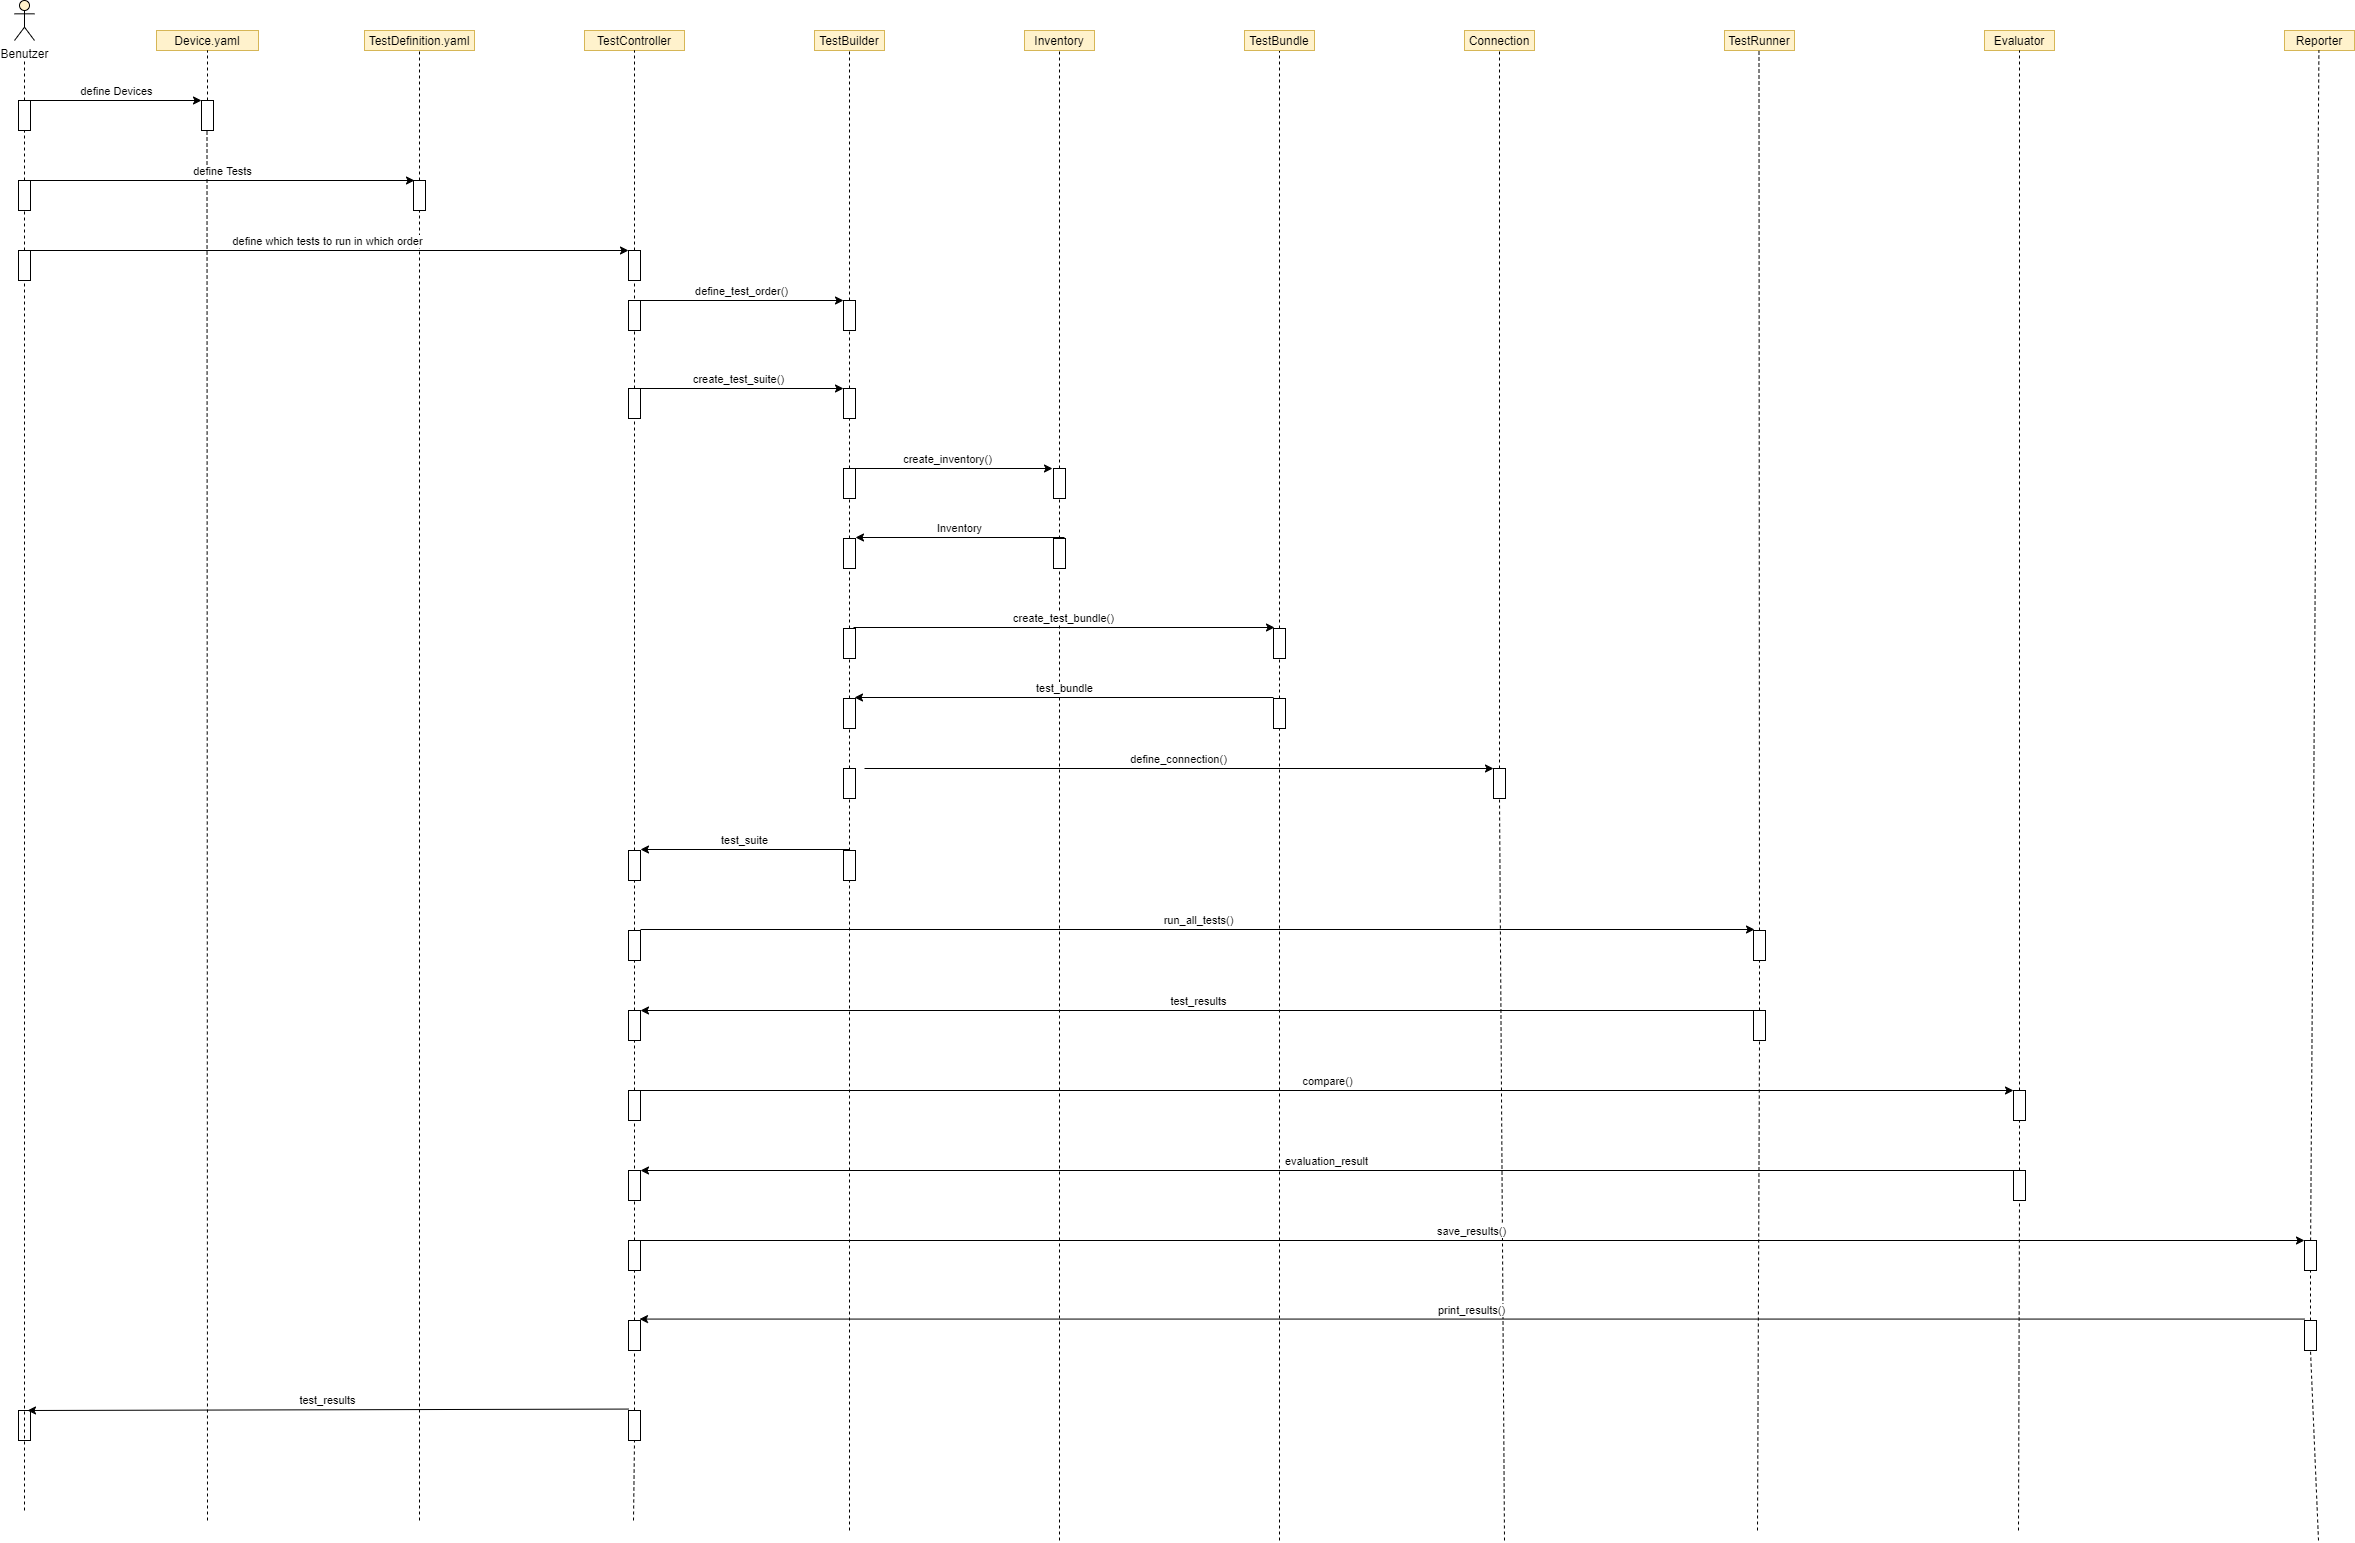
\includegraphics[scale=0.25]{\vorlagenOrdner/Bilder/SystemSSD}
		\caption{Systemsequenzdiagramm}
	\end{figure}
		\newpage
\end{landscape}
	
	\subsubsection{TestBundle}
	\begin{figure}[h!]
		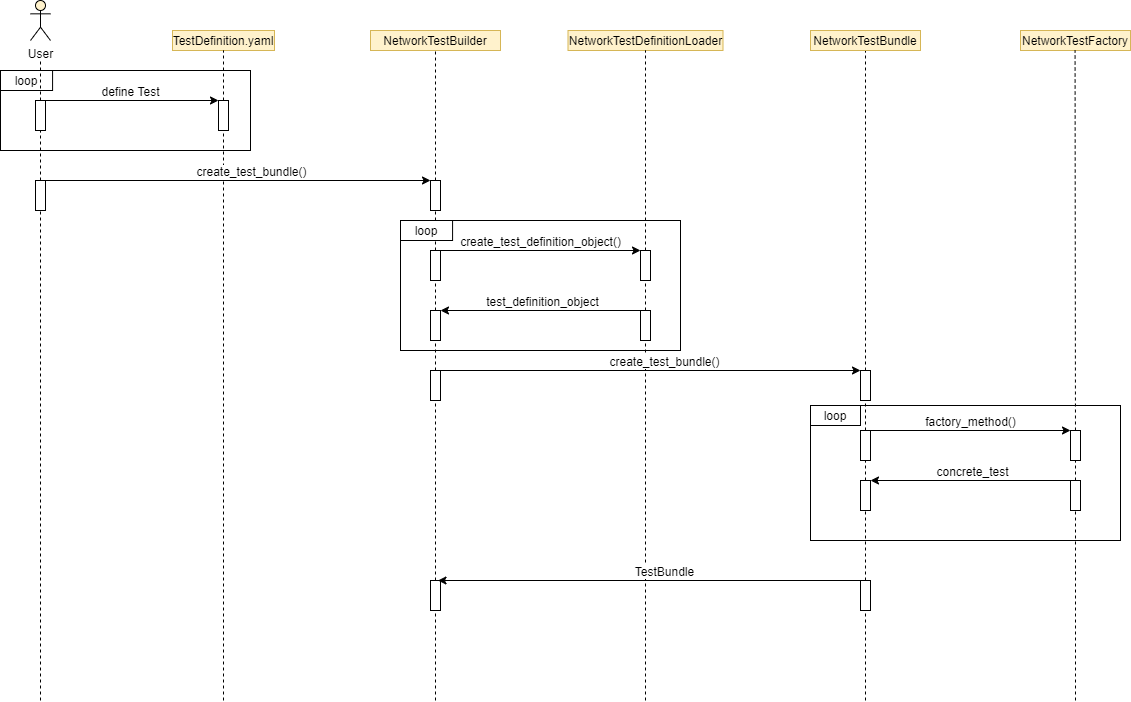
\includegraphics[scale=0.35]{\vorlagenOrdner/Bilder/TestSSD}
		\caption{TestBundle Sequenzdiagramm}
	\end{figure}

	\newpage
	
	\subsubsection{Inventar}
	\begin{figure}[h!]
		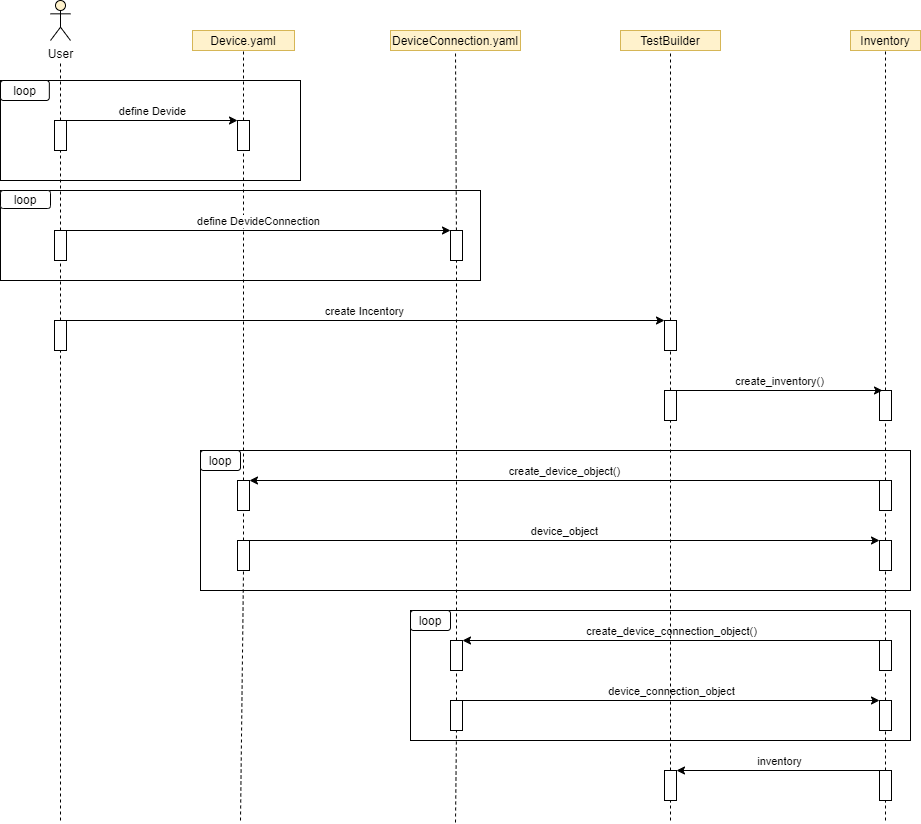
\includegraphics[scale=0.5]{\vorlagenOrdner/Bilder/InventorySSD}
		\caption{Inventar Sequenzdiagramm}
	\end{figure}

	\newpage

	\subsubsection{Connection}
	\begin{figure}[h!]
		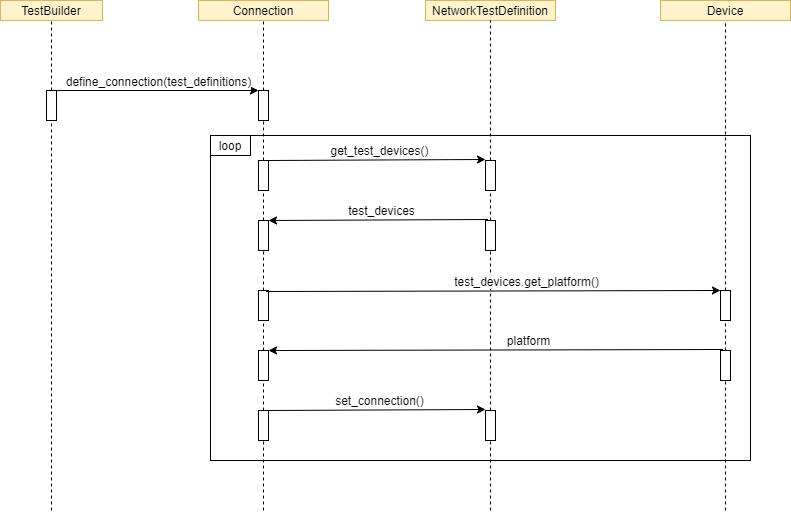
\includegraphics[scale=0.5]{\vorlagenOrdner/Bilder/ConnectionSSD}
		\caption{Connection Sequenzdiagramm}		
	\end{figure}
		
\end{document}
